
前節までで、SCALEのコンパイル方法を説明した.ここでは前節までのコンパイルが正常に終了し,

\begin{verbatim}
  scale-les/test/tutorial/bin
\end{verbatim}
にscale-les,scale-les\_init,scale-les\_ppが生成されているもととして,このチュートリアル(その1)では理想実験の例を示す.
なお,理想化実験の実験セットは

\begin{verbatim}
  scale-les/test/case
\end{verbatim}
に以下に複数用意されているが,このチュートリアルでは,4MPIプロセスで実行できるSUPERCELLの実験事例を紹介する.
正常に実験が終了した場合,図\cite{fig3.1}のような鉛直断面の画像が出力される.
なお,現実事例を想定したNestingによる実験については次節を参照されたい.

\subsection{実行方法}
チュートリアルのための,理想実験は,
\begin{verbatim}
  scale-les/test/tutorial/ideal/tutorial
\end{verbatim}
にて実行する.このチュートリアルにおいては,このディレクトリの中で前節までに生成された実行バイナリにリンクを張り,それを実行する.
実行するためには,まず上記のディレクトリに移動する.

\begin{verbatim}
  $ cd scale-les/test/tutorial/ideal/tutorial
\end{verbatim}
このディレクトリに於いて,tutorial\_test.shを実行することで,4MPI並列にて「初期値作成」,および「実験の実行」を行う.
この際行われる実験では,HEVI,1-moment雲微物理モデルを用いた計算を行う(放射やサブグリッドスケールモデルは考慮しない).

\begin{verbatim}
  $ sh tutorial_test.sh
\end{verbatim}

Core i7搭載のiMacにて,計算におおよそ15分程度程度を要する.正常に終了すると,t=600, 1200, 1800, 2400[sec]のx-z断面が順次描画される.
この描画にはgphysが必要なため,gphysが正しくインストールされている必要がある.図\cite{fig3.1}はt=1200[sec]の鉛直断面である.

\begin{figure}[t]
\begin{center}
  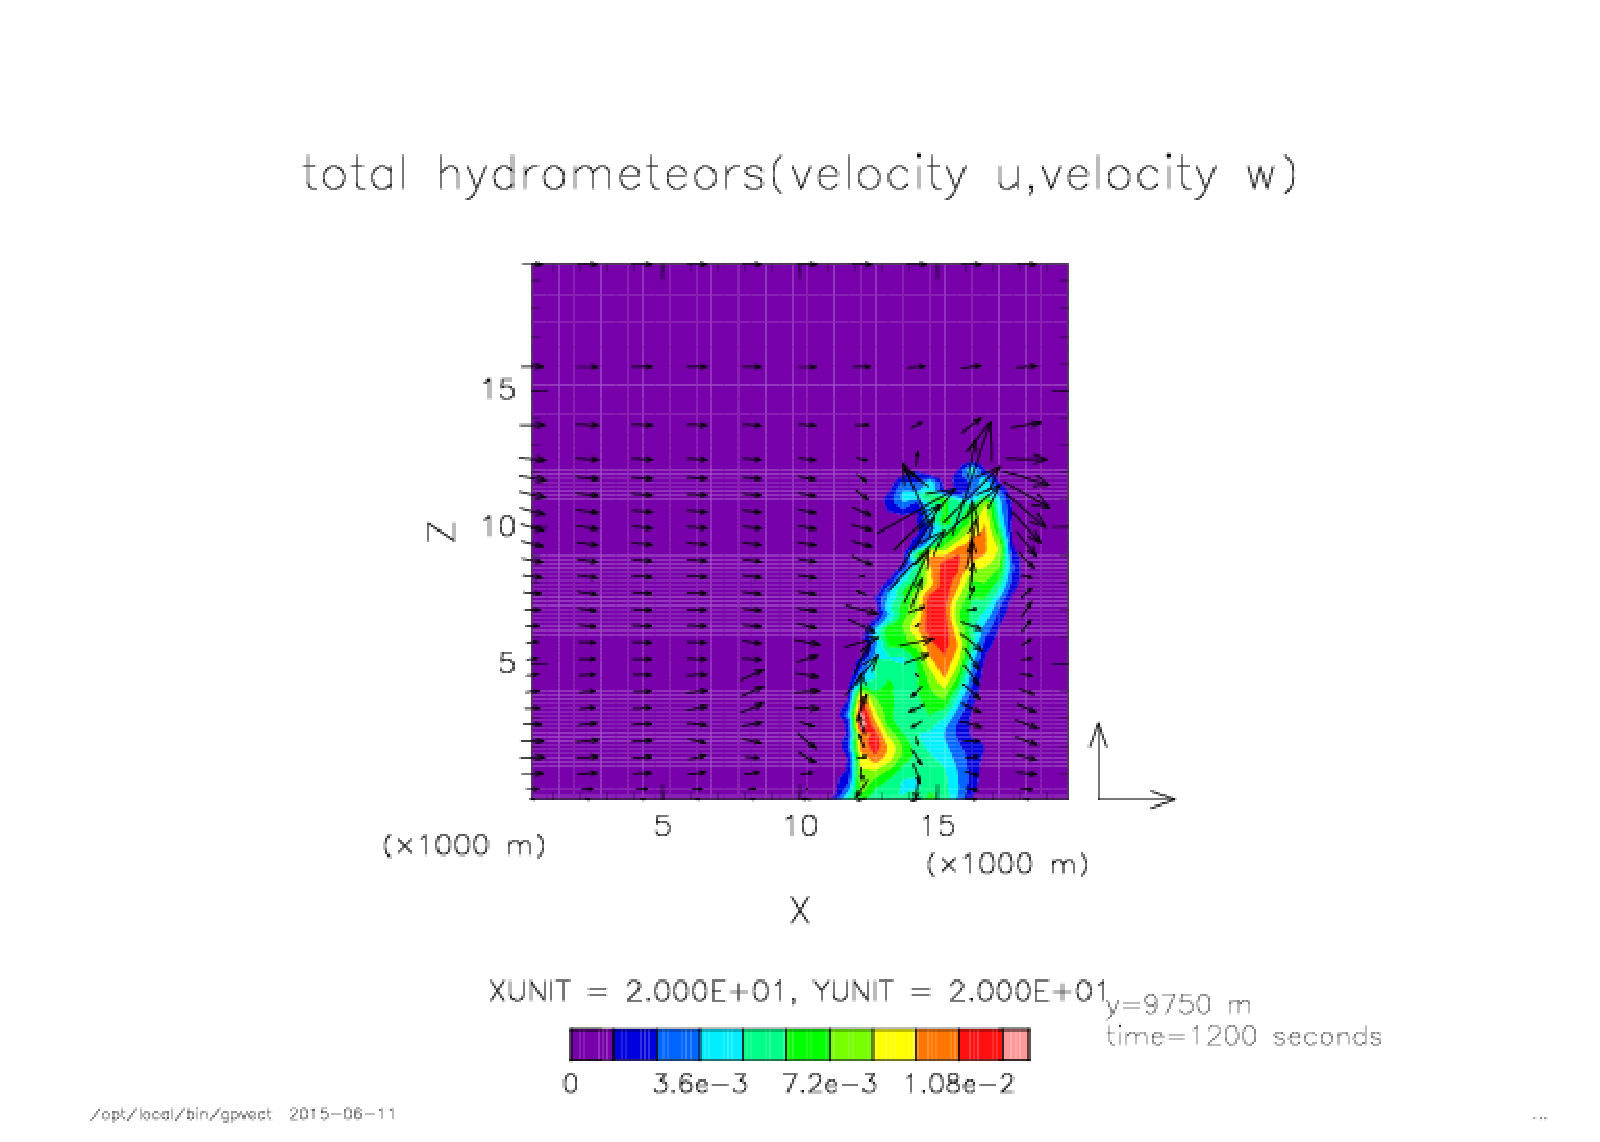
\includegraphics[width=0.9\hsize]{./figure/gpview_hist_ideal.eps}\\
  \caption{$CASE=3$を選択した際の,t=1200secにおける,y=10kmの水物質混合比のx-z断面(シェード)と風速(矢羽)}
  \label{fig3.1}
\end{center}
\end{figure}

なお,この方法では,20km x 20km x 20km(解像度はdx=dy=500m)の3次元の実験を行うが,
\begin{verbatim}
  tutorial_test.sh
\end{verbatim}
をviなどのエディタで開き,最上部にあるCASEの値を1〜5に変更することで,2次元の実験や,解像度を変更した実験や,
雲微物理モデルを2-moment bulk雲モデルを用いた実験を行うことができる.CASEを1〜5に設定した際のそれぞれの意味は
tutorial\_test.shの中の,CASEの直下に書かれている説明書きを参照されたい.

\subsection{実験の詳細}
次に上記シェルを実行した際に行われたことを説明しながら,SCALEを用いて理想化実験を行う方法を説明する.
viなどのエディタで開くと,tutorial\_test.shは,

\begin{enumerate}
\item 実行に必要な設定ファイル(init.conf,run.conf),および実行バイナリにリンクを張る
\item ジョブを実行するシェル(run.sh)を作成し(make jobshell),実行する(sh run.sh).
\item リンクを削除する
\item 描画する
\end{enumerate}

の4つの部分に分かれていることがわかる.SCALEの操作に慣れてきたら2の「ジョブ実行するシェルの実行」のみの
処理で実験を行うことができるようになる.実際にジョブを実行するシェル(run.sh)をviなどのエディタで開くと,このシェルでは

\begin{enumerate}
\item 初期値の作成(mpirun -np *** scale-les\_init init.conf)
\item 実験の実行(mpirun -np *** scale-les run.conf)
\end{enumerate}

の2つの処理が行われている.1:初期値作成の詳細な設定はinit.conf(実際にはCASEの設定で選択されたそれぞれのinit\_***.conf)で行う.
2:実験の実行時の詳細な設定はrun.conf(実際にはCASEの設定によって選択されたそれぞれのrun\_***.conf)で行う.
init.confに書かれているNamelistを編集することで,様々な実験の初期設定をすることができ,実験の詳細な設定はrun.confを編集することで
可能になる.run.confおよびinit.confに含まれるNamelistの詳細はAppendiex\cite{appendixA2}を参照されたい.\\

また,上記のチュートリアルでは,tutorial\_test.shを実行することで、run.confとinit.confにリンクを張って,実行し,描画するという一連の
処理を行ってきたが,各ユーザーの行いたい実験設定に合わせたrun.confやinit.confを作成し,run.shを実行することで,各ユーザーが行いたい
実験を行うことが可能になる.以下では,本チュートリアルで行った実験を例にして,解像度,計算領域のサイズ,物理モデルを仕様する手続き,
実行時間の変更方法などを説明していくが,ここでは,テンプレートとしてCASE=3を選択した時に利用したrun\_R40kmDX500m.confと
init\_R40kmDX500m.confをテンプレートとしてinit.confとrun.confを用意しておく.例えば

\begin{verbatim}
 cp run\_R40kmDX500m.conf. run.conf
 cp init\_R40kmDX500m.conf init.conf
\end{verbatim}

のようにして,あらかじめrun.confとinit.confをしておく.その後以下に示すような変更をrun.confやinit.confに加え,実行バイナリにリンクを張る
その上で

\begin{verbatim}
 sh run.sh 
\end{verbatim}

として実験設定を変更した計算を実行することができる.

\textcolor{red}{\large ここに出力ファイルの形式についての説明を加える;
init, history, restartが出力されること、NetCDF/CF形式、領域分割であることを説明する。}

\subsection{解像度,計算領域のサイズの設定方法}
解像度、および問題サイズは,init.conf,run.confのPARAM\_PRC,PARAM\_INDEX,PARAM\_GRIDに設定する.この際に

\underline{{\bf init.confとrun.confのPARAM\_PRC,PARAM\_INDEX,PARAM\_GRIDは}}\\
\underline{{\bf 必ず同一になる必要がある}}\\
ことに注意されたい.\\

\subsubsection{解像度}
解像度は,PARAM\_GRIDのDX,DY,DZによって格子間隔を設定する場合と,または直接グリッドの位置を指定することで設定する.\\
格子間隔を指定する場合は,PARAM\_GRIDにDX=xxx(単位は[m])のように設定する.x方向はDX,y方向はDY,z方向はDZで設定する.
この際,BUFFER\_DX,BUFFER\_DY,BUFFER\_DZ,BUFFFACTによって計算領域の両端(水平方向)とモデル上端に入れるスポンジ層を設定する.
BUFFER\_DX(BUFFER\_DY,BUFFER\_DZ)は,それぞれの方向のスポンジ層の厚さを示す.この方法で設定した場合スポンジ層の始まる層から
計算領域の端に向かって徐々に層は厚くなる.BUFFFACTによってスポンジ層を何層設けるかが決まる.BUFFFACTと層厚との関係は

\begin{eqnarray}
(DX)_{i_{sponge}+1}=(DX)_{i_{sponge}}^{BUFFFACT}
\label{eq3.1}
\end{eqnarray}

のようになる.ここで$i_{sponge}$はスポンジ層内のグリッド番号である.この関係を満たすようにスポンジ層の厚さが決まる.\\
グリッド幅を直接与える場合はFZ(:)=***(層数分のデータ,単位は[m])のように与える(FZはグリッドのFACEの位置を表す).
init\_R40kmDX500m.confを例にとると,水平解像度はDX,DYで指定し,水平方向にはスポンジ層はなく,鉛直解像度はFZを直接
記述する形で指定されている.同時にrun\_R40kmDX500m.confにおいても同一の値が設定されていることも確認されたい.


\subsubsection{問題サイズ}
問題サイズの設定はプロセス数と1MPIプロセスあたりが計算する格子点数によって設定する.1MPIプロセスあたりが計算する
格子点数はPARAM\_INDEXに記載される,KMAX,IMAX,JMAXによって決まる.これらはそれぞれ,1MPIプロセスが計算する
鉛直(z)方向,x方向,およびy方向の格子点数を示す.\\
これらに加えてPARAM\_PRCに記載されているPRC\_NUM\_X,PRC\_NUM\_Yよって問題サイズを決める.
理想化実験においては,SCALEは領域を水平分割してMPI並列計算を行う.PRC\_NUM\_X,PRC\_NUM\_Yはそれぞれ,X方向,Y方向
の分割数を示す.そのため,x方向の総格子点数はPRC\_NUM\_X$\times$IMAX,y方向の総格子点数はPRC\_NUM\_Y$\times$JMAXとなる.\\
実験に用いる総MPIプロセス数はPRC\_NUM\_X$\times$PRC\_NUM\_Yとなるため,実験を実行する際の実行シェル(run.sh)に記載された
実行時の総プロセス数とPRC\_NUM\_X$\times$PRC\_NUM\_Yは同一でなければならない.例えばPRC\_NUM\_X=2,PRC\_NUM\_Y=2の場合は
下記のように実行時の総プロセス数を4(=2 $\times $ 2)としなければならない。

\begin{verbatim}
  mpirun -np 4 scale-les run.conf
\end{verbatim}

この条件を満たさない場合は,LOGファイルなどに\\
\fbox{xxx total number of node does not match that requested. Check!}\\

という出力がされて,計算が進むことなく終了する.\\
上記で示した1MPIプロセスあたりが計算する格子点数と,x,y方向の分割数の設定によって問題サイズを設定することができる.
例えば,水平,鉛直500mの解像度(一様)で,20km $\times$ 20km $\times$ 20kmを網羅した計算を4MPI並列で行う場合
(スポンジ層はなし)は, 

\begin{verbatim}
  DX=500.D0
  DY=500.D0
  DZ=500.D0
  KMAX=40
  IMAX=20
  JMAX=20
  PRC_NUM_X=2
  PRC_NUM_Y=2
\end{verbatim}

のように設定する.さらに,同じ解像度で,x方向のみ計算領域を2倍にする場合は下記のように設定すればよい.

\begin{verbatim}
  DX=500.D0
  DY=500.D0
  DZ=500.D0
  KMAX=40
  IMAX=20 (IMAX=40)
  JMAX=20
  PRC_NUM_X=4 (PRC_NUM_X=2)
  PRC_NUM_Y=2
\end{verbatim}

ここで,括弧外で書かれた設定も,括弧内で書かれた設定も,計算ドメインのサイズと,解像度は同じである.
しかしながら,括弧外の場合は8MPIプロセス,括弧内の場合は4MPIプロセスで計算を行う.どちらを選択するかは,
それぞれが所有する計算資源によって決めるのがよい.また,同じ計算ドメインのサイズで,水平解像度を2倍にする場合は,

\begin{verbatim}
  DX=250.D0
  DY=250.D0
  DZ=500.D0
  KMAX=40
  IMAX=40 (IMAX=20)
  JMAX=40 (JMAX=20)
  PRC_NUM_X=2 (PRC_NUM_X=4)
  PRC_NUM_Y=2 (PRC_NUM_Y=4)
\end{verbatim}

のように設定する.括弧内,括弧外どちらの設定でもよい.また,モデル上端に200m程度のスポンジ層を設ける場合は,

\begin{verbatim}
  DX=250.D0
  DY=250.D0
  DZ=500.D0
  KMAX=40
  IMAX=40 (IMAX=20)
  JMAX=40 (JMAX=20)
  PRC_NUM_X=2 (PRC_NUM_X=4)
  PRC_NUM_Y=2 (PRC_NUM_Y=4)
  BUFFER_DZ=200.d0
  BUFFFACT = 1.1d0
\end{verbatim}

のように設定する.上記の\cite{eq3.1}を参考にBUFFFACTを調整することで,スポンジ層が何層になるかを設定できる.\\

\subsubsection{側面境界条件}
また,理想実験にて,水平方向にスポンジ層を設定しない場合は側面境界条件を周期境界条件を用いなければ人工的な
波が反射するなどして,計算結果に影響を及ぼす.そのため,理想化実験においてデフォルトでは周期境界条件が適用されている.
周期境界条件をやめ,開放条件で実験する際はinit.conf,run.confの中にあるNamelist,PARAM\_PRCに

\begin{verbatim}
 PRC_PERIODIC_X  = .false.,
 PRC_PERIODIC_Y  = .false.,
\end{verbatim}

と加える(どちらの変数もデフォルトはtrueで周期境界が用いられる).スポンジ層ではレイリーダンピングがかけられる.
スポンジ層でかけるレイリーダンピングの設定はrun.confのPARAM\_ATMOS\_BOUNDARYで設定する.
設定方法の一例とそれぞれのNamelistの意味を下に示す.

\begin{verbatim}
 ATMOS_BOUNDARY_TYPE         = "INIT",  (初期値に近づくように緩和する)
 ATMOS_BOUNDARY_USE_VELZ     = .true., (速度の鉛直成分にダンピングを適用する)
 ATMOS_BOUNDARY_USE_VELX     = .true., (速度のx成分にダンピングを適用する)
 ATMOS_BOUNDARY_USE_VELY     = .true., (速度のy成分にダンピングを適用する)
 ATMOS_BOUNDARY_USE_POTT     = .true., (温位にダンピングを適用する)
 ATMOS_BOUNDARY_USE_QV       = .true., (温位にダンピングを適用する)
 ATMOS_BOUNDARY_TAUX         =  300.D0, (x方向のダンピングの時定数:300[sec])
 ATMOS_BOUNDARY_TAUY         =  300.D0, (y方向のダンピングの時定数:300[sec])
 ATMOS_BOUNDARY_TAUZ         =  10.D0,  (z方向のダンピングの時定数:300[sec])
\end{verbatim}

各Namelistの詳細はAppendixを参照されたい.

\subsubsection{計算時間とdtの設定}
上記の実験では1時間(3600秒)分の時間積分を力学のタイムステップ0.6秒,雲物理のタイムステップ3.0秒で行った.
積分時間を伸ばしたい場合や,タイムステップの長さの感度を確認する場合にはタイムステップを変更する必要がある.
それらの時間はrun.confに含まれるNamelistのPARAM\_TIMEで設定する.以下に例としてtutorial\_test.shで
CASE=3を選択した際に使用されるrun\_R20kmx20kmDX500m.confの例を示す.

\begin{verbatim}
 TIME_STARTDATE             = 0000, 1, 1, 0, 0, 0, (計算開始の日付:放射スキームを用いる時や現実場を仮定した実験で必要)
 TIME_STARTMS               = 0.D0, (計算開始時刻[mili sec])
 TIME_DURATION              = 3600.0D0, (積分時間[単位はTIME_DURATION_UNITで決定])
 TIME_DURATION_UNIT         = "SEC", (積分時間TIME_DURATIONの単位)
 TIME_DT                    = 3.0D0, (トレーサー移流のタイムステップ)
 TIME_DT_UNIT               = "SEC", (TIME_DTの単位)
 TIME_DT_ATMOS_DYN          = 0.6D0, (力学のタイムステップ)
 TIME_DT_ATMOS_DYN_UNIT     = "SEC", (TIME_DT_ATMOS_DYNの単位)
 TIME_DT_ATMOS_PHY_MP       = 3.0D0, (雲物理のタイムステップ)
 TIME_DT_ATMOS_PHY_MP_UNIT  = "SEC", (TIME_DT_ATMOS_PHY_MPの単位)
\end{verbatim}

上記の各部分を変更することで積分時間,タイムステップを変更することができる.

\subsection{物理モデルの利用}
ここまで,モデルの実行方法およびと描画,および計算領域の設定などを行ってきた.本節では.物理モデル
(雲物理,乱流スキームなど)の利用方法を説明する.まず,上記の実験で用いてきた物理モデルなどを知るために,
run.conf(例としてtutorial\_test.shでCASE=3を選択した際に使用されるrun\_R20kmx20kmDX500m.conf)を再度確認する.


\subsubsection{雲微物理スキームの変更}
チュートリアルでは,Tomita (2008)の1-momentバルク法を用いていたが,SCALEには暖かい雲のみを考慮する1-momentバルク法(Kessler 1969),
氷雲を含んだ2-momentバルク法(Seiki and Nakajima, 2014),1-momentビン法の4種類の雲微物理スキームを利用することが可能である.これらの
雲微物理スキームの選択は,init.confとrun.confに記載されているPARAM\_TRACERに含まれる「TRACER\_TYPE」及び,PARAM\_ATMOSに含まれる
「ATMOS\_PHY\_MP\_TYPE」によって設定する.{\bf 両者は同じにする必要があり},選択する雲微物理スキームによって以下のように設定する.

\begin{verbatim}
KESSLER :水雲のみの1-momentバルク法(Kessler 1969)
TOMITA08:氷雲を含む1-momentバルク法(Tomita 2008)
SN14    :氷雲を含む2-momentバルク法(Seiki and Nakajima 2014)
SUZUKI10:1-momentビン法(Suzuki et al. 2010,氷雲を含むか否かはオプションで選択)
\end{verbatim}

このとき\\
\underline{{TRACER\_TYPEとATMOS\_PHY\_MP\_TYPEはinit.conf,run.confで同一にする必要がある}}\\
ことに注意されたい.\\
SUZUKI10以外を選択した場合は,init.conf,run.confのTRACER\_TYPEとATMOS\_PHY\_MP\_TYPEを変更してrun.shを実行(sh run.sh)すれば,
チュートリアルと同様に実験が実行される.一方SUZUKI10を選択した時は,init.conf,run.confの双方に

\begin{verbatim}
&PARAM_BIN
 nbin   = 33, (ビンの数)
 ICEFLG =  1, (氷雲を考慮するか否か,0->水雲のみ,1->氷雲も含む)
/
\end{verbatim}

を追記し,さらに,init.confに記載されているPARAM\_MKINITに「flg\_bin = .true. 」を追加する必要がある.

\begin{verbatim}
&PARAM_MKINIT
 flg_bin = .true.
/
\end{verbatim}

この時も,{\bf init.confとrun.confに記載されるPARAM\_BINは同一にする必要がある}.SUZUKI10を選択した時には,micpara.datという
雲微物理の計算に必要なファイルが自動生成される.micpara.datがすでに存在する場合は存在する場合はあるものを利用するが,
nbinが変わると新たに作成しなければならない.micpara.datにnbinの情報が記載されているが,もしrun.confに記載されるnbinと
micpara.datに記載されているnbinが異なれば

\fbox{xxx nbin in inc\_tracer and nbin in micpara.dat is different check!}\\

というエラーメッセージを標準出力に出力して計算が落ちるようになっている.そのため,nbinを変更した際は,micpara.datを消去して
新たに作り直す必要がある(micpara.datを消して再度SCALEをSUZUKI10を用いて実行すれば自動的に新しいmicpara.datが生成される).

\subsubsection{乱流スキームの導入}
チュートリアルでは乱流スキームは導入されていなかったが,SCALEにはSmagorinsky typeの乱流スキーム(Brown 1994, Scotti et al. 1994)と
Mellor-Yamada Level 3の乱流スキーム(MYNN, Nakanishi and Niino 2006)導入されている.これらを利用するには,init.confとrun.conf双方の
PARAM\_ATMOSに「ATMOS\_PHY\_TB\_TYPE」を加える.

\begin{verbatim}
ATMOS_PHY_TB_TYPE="SMAGORINSKY" (Smagorinsky typeのサブグリッドモデル)
ATMOS_PHY_TB_TYPE="MYNN" (Mellor-Yamada Level 3のRANSモデル)
\end{verbatim}

またrun.confのPARAM\_TIMEに

\begin{verbatim}
 TIME_DT_ATMOS_PHY_TB       = 0.10D0,  (乱流スキームの時間ステップ)
 TIME_DT_ATMOS_PHY_TB_UNIT  = "SEC", (TIME_DT_ATMOS_PHY_TBの単位)
\end{verbatim}

を加える.これらを設定した上で,run.shを実行することで,乱流スキームを考慮した計算が可能になる.
地表面フラックスのバルク係数を決めるスキーム,放射スキーム,都市スキームなどに関しては,現実事例を対象とした4章を参照されたい.

%\subsection{他の理想化実験の事例}

%この場合,デフォルトのconfigurationファイルを使用して自動的に実験設定に
%合った初期値・境界値を作成し,その後scale-lesモデル本体を実行する.
%"make run"のコマンドを使用せず,以下のように手動で実行過程を進めることもできる.
%
%\begin{enumerate}
%\item 実験設定を記述したconfigurationファイル,init.confを編集して目的の実験にあった設定を構築する.
%
%\item 下記のコマンドによって事前処理(初期値・境界値作成)を実行する.ここの例ではMPI並列として6プロセスを使用している.
%\begin{verbatim}
%$ mpirun -n 6 ./scale-les_init init.conf
%\end{verbatim}
%正常にJOBが終了すれば,
%\verb|init_****.pe#####.nc|,および\verb|boundary.pe#####.nc|
%といったファイルが,それぞれMPIプロセス数ずつ生成される(\verb|#####|はMPIプロセスの番号).
%
%\item モデルを実行するためにrun.confを適宜編集する.MPIプロセスの数や,格子,境界の取り方の設定については,init.confの時の設定と相違ないように注意すること.
%正常にJOBが終了すれば,\verb|init_****.pe#####.nc|,
%および\verb|boundary.pe#####.nc|といったファイルが,それぞれMPIプロセス数ずつ生成される(\verb|#####|はMPIプロセスの番号).
%
%\item 下記のコマンドによってモデルを実行する.
%\begin{verbatim}
%$ mpirun -n 6 ./scale-les run.conf
%\end{verbatim}
%configurationファイルの設定によるが,\verb|history.pe#####.nc|
%という名前のファイルが作成され,この中に出力変数が含まれている.
%\end{enumerate}

